\documentclass[../../lecture_notes.tex]{subfiles}
\begin{document}

\newcommand\custarr{Latex[length=3mm, width=5mm, color=white]}
The standard design for an operating system can be viewed as follows:

\begin{figure}[H]
\centering
\begin{subfigure}{0.45\linewidth}
\centering
\resizebox{\linewidth}{!}{
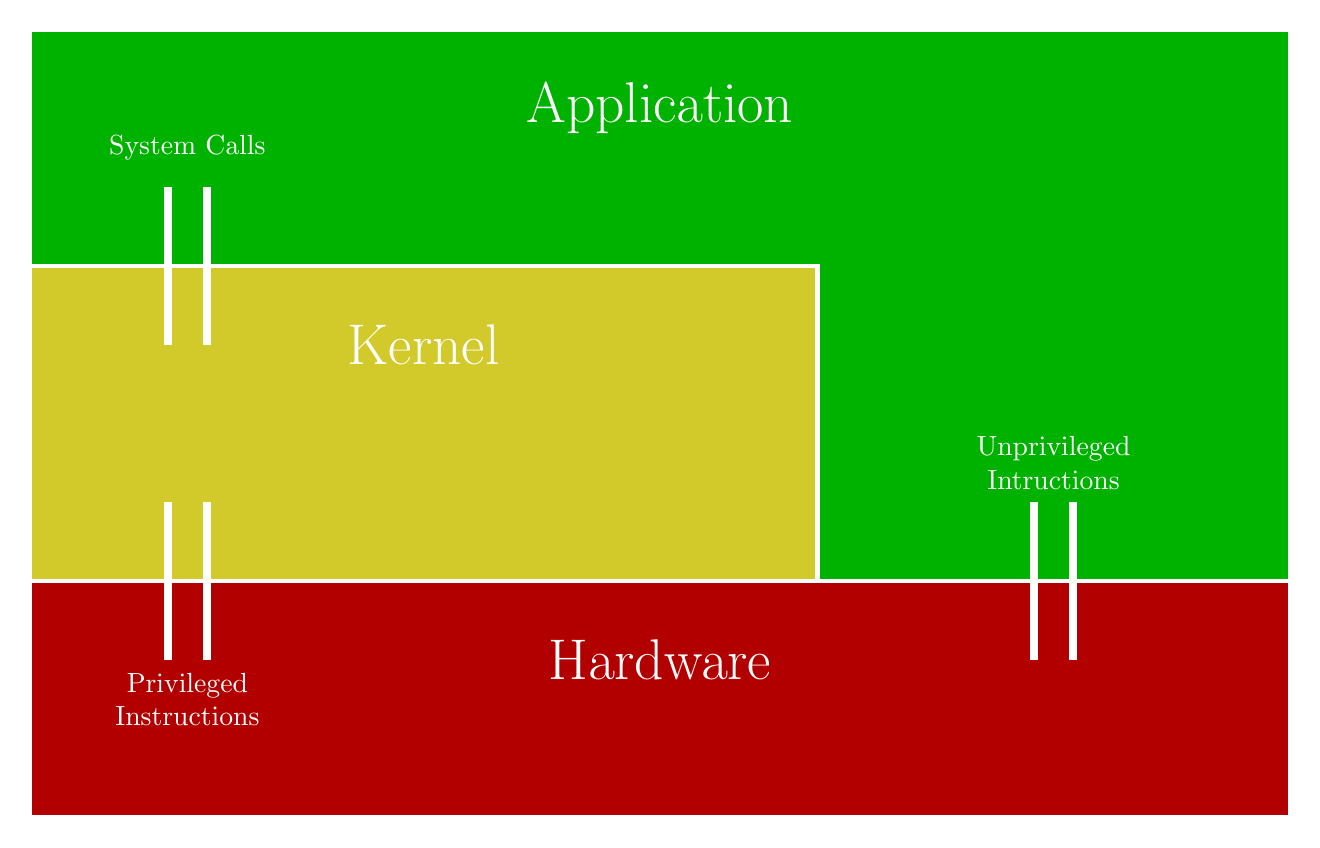
\begin{tikzpicture}
\draw[fill=black!30!green, draw=white, ultra thick] (0,0) rectangle (16,10);
\node[white, align=center] at (8,9) {\huge Application};
\draw[fill=black!20!yellow, draw=white, ultra thick] (0,3) rectangle (10,7);
\node[white, align=center] at (5,6) {\huge Kernel};
\draw[fill=black!30!red, draw=white, ultra thick] (0,0) rectangle (16,3);
\node[white, align=center] at (8,2) {\huge Hardware};

\draw[-\custarr, line width=1mm, draw=white] (1.75, 2) -- (1.75,4);
\draw[-\custarr, line width=1mm, draw=white] (2.25, 4) -- (2.25,2);
\node[align=center, white] at (2,1.5) {Privileged\\Instructions};

\draw[-\custarr, line width=1mm, draw=white] (1.75, 6) -- (1.75,8);
\draw[-\custarr, line width=1mm, draw=white] (2.25, 8) -- (2.25,6);
\node[align=center, white, thick] at (2,8.5) {System Calls};

\draw[-\custarr, line width=1mm, draw=white] (12.75, 2) -- (12.75,4);
\draw[-\custarr, line width=1mm, draw=white] (13.25, 4) -- (13.25,2);
\node[align=center, white] at (13,4.5) {Unprivileged\\Intructions};

\end{tikzpicture}
}
\caption{Course granularity view}
\end{subfigure}
~
\begin{subfigure}{0.45\textwidth}
\centering
\resizebox{\linewidth}{!}{
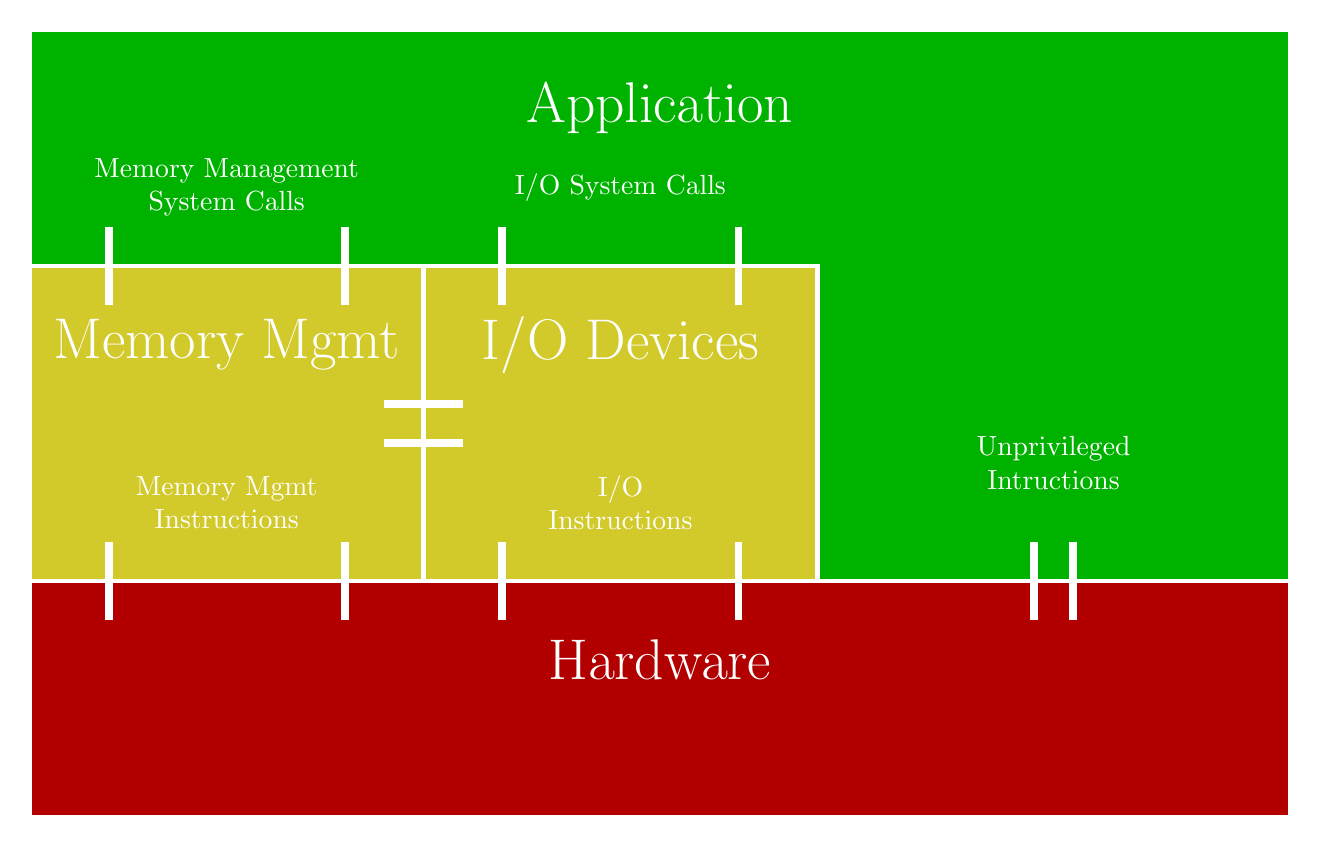
\begin{tikzpicture}
\draw[fill=black!30!green, draw=white, ultra thick] (0,0) rectangle (16,10);
\node[white, align=center] at (8,9) {\huge Application};
\draw[fill=black!20!yellow, draw=white, ultra thick] (0,3) rectangle (5,7);
\node[white, align=center] at (2.5,6) {\huge Memory Mgmt};
\draw[fill=black!20!yellow, draw=white, ultra thick] (5,3) rectangle (10,7);
\node[white, align=center] at (7.5,6) {\huge I/O Devices};
\draw[fill=black!30!red, draw=white, ultra thick] (0,0) rectangle (16,3);
\node[white, align=center] at (8,2) {\huge Hardware};

\draw[-\custarr, line width=1mm, draw=white] (1, 2.5) -- (1,3.5);
\draw[-\custarr, line width=1mm, draw=white] (4, 3.5) -- (4,2.5);
\node[align=center, white] at (2.5,4) {Memory Mgmt\\Instructions};

\draw[-\custarr, line width=1mm, draw=white] (6, 2.5) -- (6,3.5);
\draw[-\custarr, line width=1mm, draw=white] (9, 3.5) -- (9,2.5);
\node[align=center, white] at (7.5,4) {I/O\\Instructions};

\draw[-\custarr, line width=1mm, draw=white] (1, 6.5) -- (1,7.5);
\draw[-\custarr, line width=1mm, draw=white] (4, 7.5) -- (4,6.5);
\node[align=center, white, thick] at (2.5,8) {Memory Management\\System Calls};

\draw[-\custarr, line width=1mm, draw=white] (6, 6.5) -- (6,7.5);
\draw[-\custarr, line width=1mm, draw=white] (9, 7.5) -- (9,6.5);
\node[align=center, white, thick] at (7.5,8) {I/O System Calls};

\draw[-\custarr, line width=1mm, draw=white] (12.75, 2.5) -- (12.75,3.5);
\draw[-\custarr, line width=1mm, draw=white] (13.25, 3.5) -- (13.25,2.5);
\node[align=center, white] at (13,4.5) {Unprivileged\\Intructions};

\draw[-\custarr, line width=1mm, draw=white] (4.5, 5.25) -- (5.5,5.25);
\draw[-\custarr, line width=1mm, draw=white] (5.5,4.75) -- (4.5, 4.75);

\end{tikzpicture}
}
\caption{Fine granularity view}
\end{subfigure}
\end{figure}

We can see that our model has three general levels of instruction privilege:
\begin{itemize}
\item risky code with direct access to resources (OS only code) such as inb, outb
\item code that accesses resources directly some of the time (iffy code) such as movl \\ 
	(movl is privileged if memory section to be accessed is in kernel)
\item code with no access to code (unprivileged)
\end{itemize}
Untrusted modules can use code which does not have direct access; i.e. unprivileged code and (depending on context) iffy code.

To allow for these restrictions on an untrusted module, the system boots in privileged mode, sets the environment for the untrusted code, and jumps to the untrusted code in unprivileged mode. However, if the untrusted application desires access to system resources, we send an \term{interrupt} with a \term{supervisor call} instruction.

\begin{minipage}{0.2\linewidth}
\resizebox{!}{180pt}{
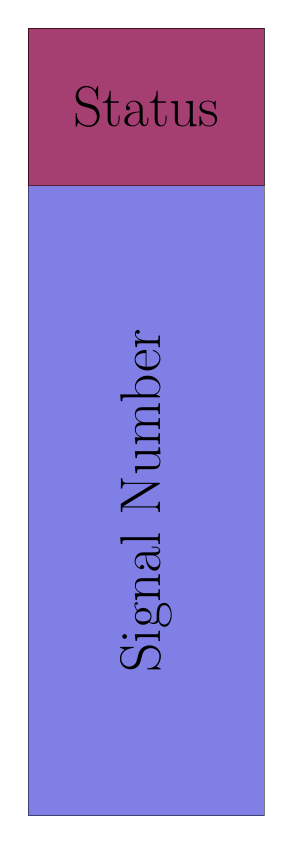
\begin{tikzpicture}
\draw[fill=black!20!blue, opacity=0.5] (0, 0) rectangle (3, 10);
\node[rotate=90, anchor=center] at (1.5, 4) {\huge Signal Number};
\draw[fill=black!20!red, opacity=0.5] (0, 8) rectangle (3, 10);
\node at (1.5, 9) {\huge Status};
\end{tikzpicture}
}
\end{minipage}%
\begin{minipage}{0.8\linewidth}
If the error code matches the error code corresponding to a given operation, the privileged instruction is run. The \term{trap} signal jumps to the kernel and raises the permission. The \term{return from trap} signal jumps to the user and lowers the permission. Trap locations are defined by \term{trap handlers}. These are held in a \term{trap table} in the kernel stack. The key for this hash table is the \term{system call number}, commonly known as the \term{interrupt number}. \smallskip

On the hardware side, when a trap occurs:
\begin{enumerate}[nosep]
\item Running program information will be pushed onto the stack.
\item \textbf{eip} will be set to interrupt service routine.
\item Stack info will be popped from the stack when \textbf{reti} is called.
\end{enumerate}
\end{minipage}

For interrupts, we can think of a processor as a hard-wired thread manager with two threads, the processor thread that runs the scheduler and the interrupt thread running in kernel mode. Threads with decreased privelage can be built on top of each other like so:

\begin{center}
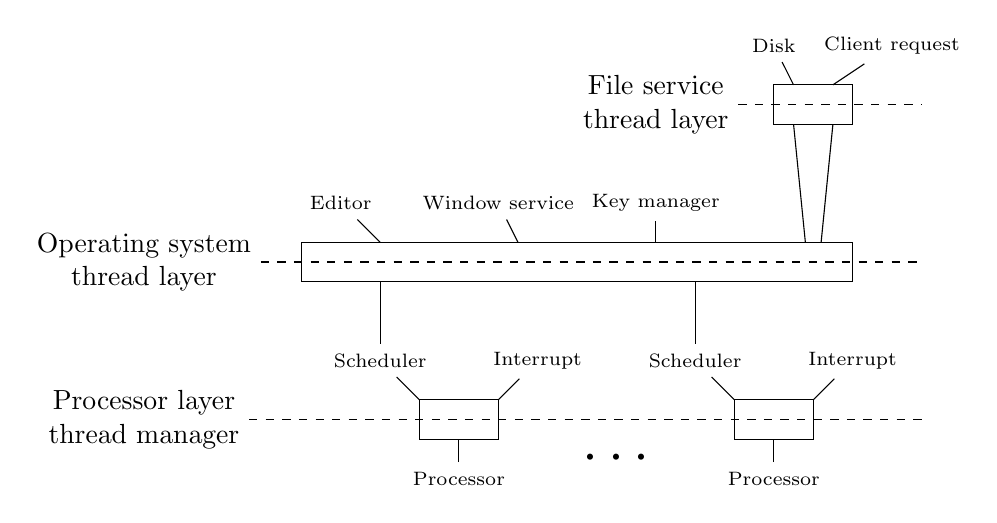
\begin{tikzpicture}
\node[align=center] at (0,0) (1) {Processor layer \\ thread manager};
\draw[draw] (3.5, -0.25) rectangle (4.5, 0.25);
\node[align=center] at (4, -0.75) (111) {\scriptsize Processor};
\draw (111) -- (4, -0.25); 
\node[align=center] at (3, 0.75) (112) {\scriptsize Scheduler};
\draw (112) -- (3.5, 0.25); 
\node[align=center] at (5, 0.75) (113) {\scriptsize Interrupt};
\draw (113) -- (4.5, 0.25); 
\node at (6, -0.5) {\huge \textbf{$\cdots$}};
\draw[draw] (7.5, -0.25) rectangle (8.5, 0.25);
\node[align=center] at (8, -0.75) (121) {\scriptsize Processor};
\draw (121) -- (8, -0.25); 
\node[align=center] at (7, 0.75) (122) {\scriptsize Scheduler};
\draw (122) -- (7.5, 0.25); 
\node[align=center] at (9, 0.75) (123) {\scriptsize Interrupt};
\draw (123) -- (8.5, 0.25); 
\node[align=center] at (10,0) (1R) {};
\draw[dashed] (1) -- (1R);

\node[align=center] at (0,2) (2) {Operating system \\ thread layer};
\draw[draw] (2, 1.75) rectangle (9, 2.25);
\draw (112) -- (3, 1.75);  \draw (122) -- (7, 1.75); 
\node[align=center] at (2.5,2.75) (21) {\scriptsize Editor}; \draw (21) -- (3,2.25);
\node[align=center] at (4.5,2.75) (22) {\scriptsize Window service}; \draw (22) -- (4.75,2.25);
\node[align=center] at (6.5, 2.75) (23) {\scriptsize Key manager}; \draw (23) -- (6.5,2.25);
\node[align=center] at (10,2) (1R) {};
\draw[dashed] (2) -- (1R);

\node[align=center] at (6.5, 4) (3) {File service\\ thread layer};
\draw[draw] (8,3.75) rectangle (9, 4.25);
\draw (8.25, 3.75) -- (8.4, 2.25); \draw (8.75, 3.75) -- (8.6, 2.25);
\node[align=center] at (8,4.75) (31) {\scriptsize Disk}; \draw (31) -- (8.25,4.25);
\node[align=center] at (9.5, 4.75) (32) {\scriptsize Client request}; \draw (32) -- (8.75,4.25);
\node[align=center] at (10,4) (1R) {};
\draw[dashed] (3) -- (1R);
\end{tikzpicture}
\end{center}


We define functions that give access to privileged instructions as \term{system calls}. This is as opposed to a \term{procedure call}, which is a function implemented on the stack that can call other functions. x86-64 Linux system calls use the convention of \%rax for the interrupt number and \%rdi, \%rsi, \%rdx, \%r10, \%r8, \%r9, in that order, for arguments.

System calls are an example of the \term{protected transfer of control}, wherein the instruction pointer is set to a location known to be safe. On x86-64, there are 2 privilege bits corresponding to 4 levels of privilege that require different amounts of protection for control transfer. These can be visualized as follows:

\begin{center}
\begin{tikzpicture}
\node[circle, fill=black!20!green, draw, minimum size=8cm] (C) at (0,0) {};
\node[circle, fill=black!20!yellow, draw, minimum size=6cm, label=above:Ring 3] at (0,0) {};
\node[circle, fill=red!50!yellow, draw, minimum size=4cm, label=above:Ring 2]  at (0,0) {};
\node[circle, fill=black!20!red, draw, minimum size=2cm, label=above:Ring 1, align=center]  at (0,0) {Ring 0};
\node[right=of C, align=center] (B) {Min Privilage};
\node[above=0cm of B, fill=black!20!green, rectangle, draw, minimum size=1cm, 
	label=right:{Applications (display, etc)}] (4) {};
\node[above=0cm of 4, fill=black!20!yellow, rectangle, draw, minimum size=1cm, 
	label=right:{Device Drivers (devices, etc)}] (3) {};
\node[above=0cm of 3, fill=red!50!yellow, rectangle, draw, minimum size=1cm, 
	label=right:{Device Drivers (memory, etc)}] (2) {};
\node[above=0cm of 2, fill=black!20!red, rectangle, draw, minimum size=1cm, 
	label=right:{Kernel}] (1) {};
\node[above=0cm of 1, align=center] {Max Privilage};
\end{tikzpicture}
\end{center}


But memory is only one thing to be protected; we must also control time access so as to avoid stalling!

\end{document}